
%\selectlanguage{english}

\section{C++ course under MicMac's library : Elise}
\subsection{Introduction and generalities}
A \verb!C++! course was organized at ENSG (The National School of Geographic Sciences). The purpose of this course is to be able to create your own programs using the Elise library used in MicMac. In this section we start by giving some information about the location of each files that will be needed, then some examples that have been implemented during this session will be detailed and explained.\newline

Here is a list of locations of files that will be used along the course:\newline
\begin{itemize}
\item $\textbf{/culture3d/src}$ : contains source files (extension .cpp) \newline
\item $\textbf{/culture3d/include}$ : contains header files (extension .h)\newline
\item $\textbf{/culture3d/include/XML\_MicMac}$ : contains \verb!xml! files describing parameters for simplified tools as \textbf{Tapioca}, \textbf{Tapas}, ... etc\newline
\item $\textbf{/culture3d/include/XML\_GEN}$ : contains \verb!xml! files, and an associated header file (generated automatically from the \verb!xml! file)\newline
\item $\textbf{culture3d/src/CBinaires/}$ : contains binaries that can be called without using \textbf{mm3d}. This is maintained, but using \textbf{mm3d} is recommended\newline
\item \textbf{mm3d.cpp} specifies each command, with some commentary and log information\newline
\end{itemize}

Some convention are used while developing MicMac tools. Here we give some of them in order to understand the approach adopted: \newline
\begin{itemize}
\item a class called toto in an \verb!xml! file will become cToto \newline
\item a member called toto in an \verb!xml! file will become mToto \newline
\end{itemize}

\subsection{How to create a new .cpp file and compile it using the library Elise?}
Start by creating a new file under the folder $\textbf{/culture3d/src/TpMMPD}$ and call it \\$\textbf{cExoMM\_CorrelMulImage.cpp}$. Note that the file $\textbf{ExoMM\_CorrelMulImage.cpp}$ under the same folder contains the solution of this course.
\subsubsection{Hello World !}
The first exercise is displaying the famous \og hello world \fg\ under the prompt. The most important thing here is to succeed to compile your directory \textbf{culture3d} with your new file  $\textbf{cExoMM\_CorrelMulImage.cpp}$.\newline


Under your favorite IDE, for example Geany, start by including this file \textbf{StdAfx.h} which contains all the headers of the library Elise. You are invited to check what is contained under $\textbf{/culture3d/include/StdAfx.h}$ \newline

\begin{lstlisting}
#include "StdAfx.h"

int ExoMCI_main(int argc, char ** argv)
{
     std ::cout << "hello world" << "\n";
     return EXIT_SUCCESS;
}
\end{lstlisting}

\textbf{\textcolor{red}{Achtung !}} We need to tell the compiler that there is a new source file.

Edit \textbf{Source.cmake} under the same folder and add this line : \newline

\begin{verbatim}
set(Src_TD_PPMD ${TDPPMD_DIR}/cExoMM_CorrelMulImage.cpp
\end{verbatim}

You also need to comment this line while your are doing this tutoriel:
\begin{verbatim}
#${TDPPMD_DIR}/ExoMM_CorrelMulImage.cpp
\end{verbatim}

In order to call our program we need to add in \textbf{culture3d/src/CBinairies/mm3d.cpp} the following line: \newline

\begin{verbatim}
aRes.push_back(cMMCom("ExoMCI",ExoMCI_main,"Exo: Multi Correlation Image"));
\end{verbatim}

This line should be added under : \newline
\begin{verbatim}
const std::vector<cMMCom> & TestLibAvailableCommands() {...}
\end{verbatim}

Check that the compilation works properly by typing as usual $\textbf{make install}$ under \og$\textbf{/culture3d/build}$\fg. Then if you type in:

\begin{verbatim}
mm3d TestLib ExoMCI
\end{verbatim}
Your prompt should display \og \textbf{hello world} \fg.\newline

 \textbf{\textcolor{red}{Achtung !}} In \textbf{/culture3d/src/CBinairies/mm3d.cpp},  \textit{getAvailableCommands()} contains a list of commands accessible through the syntax: \textbf{mm3d MyCommand}. Its declaration in the file is:
\begin{verbatim}
const std::vector<cMMCom> & getAvailableCommands() {...}
\end{verbatim}

\textit{TestlibAvailableCommands()} vector contains the commands accessible through the syntax: \textbf{mm3d TestLib MyCommand}. It's our case above.

%%%%%%%%%%%%%%%%%%%%%%%%%%%%%%%%%%%%%%%%%%%%%%%%%%%%%%%%%%%%%%%%%%
\subsection{Mandatory or Optional Argument?}
If you are a user of MicMac you know that calling a mandatory argument doesn't require to specify the name of the option. For example \textbf{Tapas} requires at least two arguments : model of distortion and a pattern, while optional arguments are specified by a name. For instance the option \textbf{InCal=} or \textbf{InOri=}.\newline


Edit $\textbf{cExoMM\_CorrelMulImage.cpp}$ and add this loop at the beginning :\newline

\begin{verbatim}
for (int aK=0; aK<argc ; aK++)
        std::cout << "Argv[" << aK << "]=" << argv[aK] << endl;
\end{verbatim}

Now, compile as before then type in the following command:
\begin{verbatim}
mm3d TestLib ExoMCI MyArg1 MyArg2
\end{verbatim}

The prompt should display:\newline

\begin{verbatim}
Argv[0] = ExoMCI
Argv[1] = MyArg1
Argv[2] = MyArg2
\end{verbatim}

\textbf{ElInitArgMain} function is used to specify which arguments are optional and which are mandatory. This function is also used to display the help. \newline

Here is a second example dealing with manipulation of arguments.\newline

Modify your file $\textbf{cExoMM\_CorrelMulImage.cpp}$ in order to contain the following code :

\begin{verbatim}
#include "StdAfx.h"

int ExoMCI_main(int argc,char ** argv)
{
     int I,J; //declaration of two  arguments
     double D=1.0; //default value (for optional args)
     ElInitArgMain
     (
          argc, argv, //list of args
          LArgMain() << EAMC(I,"Left Operand")
//EAMC means mandatory argument
                              << EAMC(J,"Right Operand"),
          LArgMain() << EAM(D,"D",true,"divisor of I+J")
//EAM means optional argument
     );

     std::cout << "(I+J)/D = " <<(I+J)/D << std::endl;

     return EXIT_SUCCESS;
}
\end{verbatim}

Compile again and type in the following command:
\begin{verbatim}
mm3d TestLib ExoMCI 1 4
\end{verbatim}

The prompt should display:
\begin{verbatim}
(I+J)/D = 5
\end{verbatim}

If you type:
\begin{verbatim}
mm3d TestLib ExoMCI 1 4 2
\end{verbatim}

Then your prompt should display:
\begin{verbatim}
(I+J)/D = 2.5
\end{verbatim}
%%%%%%%%%%%%%%%%%%%%%%%%%%%%%%%%%%%%%%%%%%%%%%%%%%%%%%%%%%%%%%%%%
\subsection{How to load an xml file and read its informations?}
Right now we will keep working with the Mini-Cuxha dataset (see \textbf{micmac\_data}). \newline

First, take a look at \og \textbf{ParamChantierPhotogram.xml}\fg. \newline
This file is under the folder \og\textbf{culture3d/include/XML\_GEN/}\fg. It describes for each object, its type, options, ... etc under an xml formalism. In the Mini-Cuxha folder, the file \textbf{120601.xml} contains ground control points. Here are the first seven lines of this file:
% OK
%\lstset {language=xml}   %%%%% to correct
\begin{verbatim}
<?xml version="1.0" ?>
<DicoAppuisFlottant>
     <OneAppuisDAF>
          <Pt>2.41677870000000006 42.595951300000003 496.235299999999995</Pt>
          <NamePt>12060100_172</NamePt>
          <Incertitude>1 1 1</Incertitude>
     </OneAppuisDAF>
\end{verbatim}

You can check if the file \og \textbf{120601.xml} \fg\ respects the formalism described in \textbf{ParamChantierPhotogram.xml}:\newline
\begin{verbatim}
   <DicoAppuisFlottant  Nb="1" Class="true">
       <OneAppuisDAF Nb="*">
           <Pt Nb="1" Type="Pt3dr"> </Pt>
           <NamePt Nb="1" Type="std::string"> </NamePt>
        <Incertitude Nb="1"  Type="Pt3dr"> </Incertitude>
       </OneAppuisDAF>
   </DicoAppuisFlottant>
\end{verbatim}

\textbf{Nb} parameter can be set to :
\begin{itemize}
\item 1 : this tag should appear once
\item ? : this tag can appear once, but it's not mandatory
\item * : there can be given as many of these tags \newline
\end{itemize}

\textbf{Type} parameter is a classical \verb!C++! type class, indeed some of MicMac's classes, as for instance: Pt3dr means a real 3D point, Pt2di means a 2D integer point, ... etc. \newline

The function $\textbf{StdGetFromPCP(aStr,aObj)}\footnote{PCP means ParamChantierPhotogram.h}$ describes how to link the xml file to its description. You can check $\textbf{/culture3d/include/private/files.h}$ for more details. \newline

Now, edit $\textbf{cExoMM\_CorrelMulImage.cpp}$ in order to contain the following code:
% NOT OK
\begin{verbatim}
#include "StdAfx.h"

int ExoMCI_main(int argc,char ** argv)
{
     std::string aNameFile; //will store your xml filename
     double D=1.0; //default value for optional argument
     ElInitArgMain //displays the help, and affect your command line to members
     (
          argc, argv, /arguments list
          LArgMain() << EAMC(aNameFile,"Left Operand"), //EAMC = mandatory argument
          LArgMain() << EAM(D,"D",true,"Unused") //EAM = optional argument
     );

     //the DicoAppuisFlottant (xml file) is converted to cDicoAppuisFlottant (c++)
     cDicoAppuisFlottant aDico= StdGetFromPCP(aNameFile,DicoAppuisFlottant);

     std::cout << "NbPts = " << aDico.OneAppuisDAF().size() << std::endl;

     return EXIT_SUCCESS;
}
\end{verbatim}

Try to compile again an typing the following command :
\begin{verbatim}
mm3d TestLib ExoMCI 120601.xml
\end{verbatim}

Your prompt should display : NbPts = 11 \newline

If you want to access to each individual element and display for instance the name and coordinates for each point, you should add a loop and browser each \textbf{OneAppuisDAF} like following:

\begin{verbatim}
std::list<cOneAppuisDAF> & aLGCP =  aDico.OneAppuisDAF();
         //OneAppuisDAF (xml) becomes cOneAppuisDAF (C++)
     for ( //as long as we are in the same dictionnary ==> browse each point
          std::list<cOneAppuisDAF>::iterator iT = aLGCP.begin();
          iT != aLGCP.end();
          iT++ )
          {
          std::cout << iT->NamePt() << " " << iT->Pt() << "\n";
          //NamePt and Pt are the classes names in the xml
          }
\end{verbatim}
%%%%%%%%%%%%%%%%%%%%%%%%%%%%%%%%%%%%%%%%%%%%%%%%%%%%%%%%%%%%%%%%%%%%%%%%%%%%%%
\subsection{How to get list of files in a folder?}
Here we start by declaring and defining two classes that we will use later in our global exercise which contains the algorithm of Multi Correlation Images. Our first class $\textbf{cMCI\_Appli}$ concerns the application, and the second one $\textbf{cMCI\_Ima}$ deals with image manipulations and will be defined in next section. \newline

Now, edit again your file $\textbf{cExoMM\_CorrelMulImage.cpp}$ in order to contain the following code:

\begin{verbatim}
#include "StdAfx.h"

//list of class
class cMCI_Appli;
class cMCI_Ima;

//classes declaration
class cMCI_Appli
{
     public :
          cMCI_Appli(int argc,char ** argv);
     private :
          std::list<std::string> mLFile;
          std::string mFullName;
          std::string mDir; //directory in which we are working
          std::string mPat; //pattern of images
          cInterfChantierNameManipulateur * mICNM;
};

cMCI_Appli::cMCI_Appli(int argc,char ** argv)
{
     bool aShowArgs=true;
     ElInitArgMain
     (
          argc, argv, //list of args
          //EAMC = mandatory argument
          LArgMain() << EAMC(mFullName,"Full Name (Dir+Pat)"),
          //EAM = optional argument
          LArgMain() << EAM(aShowArgs,"Show",true,"Gives details on arguments")
     );

     SplitDirAndFile(mDir, mPat, mFullName);
     mICNM = cInterfChantierNameManipulateur::BasicAlloc(mDir);
     mLFile = mICNM->StdGetListOfFile(mPat);

     if (aShowArgs) ShowArgs();
}

void cMCI_Appli::ShowArgs()
{
     std::cout << "DIR = " << mDir << "Pat = " << mPat << "\n";
          std::cout << "Nb Files " << mLFile.size() << "\n";
          for (
               std::list<std::string>::iterator itS=mLFile.begin();
               itS != mLFile.end();
               itS ++)
                    { std::cout << "     F = " << *itS << "\n"; }

}
int ExoMCI_main(int argc,char ** argv)
{
     cMCI_Appli anAppli(argc,argv);
     return EXIT_SUCCESS;
}
\end{verbatim}

Try to compile and from the \textbf{Mini-Cuxha} folder type in the following command:
\begin{verbatim}
mm3d TestLib ExoMCI ".*jpg"
\end{verbatim}

Your prompt should display:
\begin{verbatim}
Nb Files 48
     F = Abbey-IMG\_0173.jpg
     F = Abbey-IMG\_0191.jpg
\end{verbatim}

\subsection{Epipolar geometry}
Here, first we need to create a couple of images with an epipolar rectification. In the directory \textbf{Mini-Cuxha}, we can use the tool \textbf{mm3d CreateEpip} for completing this. If the name of our orientations computed is \textbf{RTL-Init}, type in the following command gives our couple of images needed:
\begin{verbatim}
mm3d CreateEpip Abbey-IMG_0173.jpg Abbey-IMG_0191.jpg RTL-Init
\end{verbatim}

Then, edit your file $\textbf{cExoMM\_CorrelMulImage.cpp}$ in order to contain the following code:
\begin{verbatim}
#include "StdAfx.h"

int  ExoMCI_main(int argc,char ** argv)
{
    std::string aNameI1,aNameI2;
    int aPxMax= 199;
    int aSzW = 5;
    ElInitArgMain
    (
        argc,argv,
        LArgMain()  << EAMC(aNameI1,"Name Image1")
                    << EAMC(aNameI2,"Name Image2"),
        LArgMain()  << EAM(aPxMax,"PxMax",true,"Pax Max")
    );

    Im2D_U_INT1 aI1 = Im2D_U_INT1::FromFileStd(aNameI1);
    Im2D_U_INT1 aI2 = Im2D_U_INT1::FromFileStd(aNameI2);

    Pt2di aSz1 = aI1.sz();
    Im2D_REAL4  aIScoreMin(aSz1.x,aSz1.y,1e10);
    Im2D_REAL4  aIScore(aSz1.x,aSz1.y);
    Im2D_INT2   aIPaxOpt(aSz1.x,aSz1.y);

    Video_Win aW = Video_Win::WStd(Pt2di(1200,800),true);

    for (int aPax = -aPxMax ; aPax <=aPxMax ; aPax++)
    {
        std::cout << "PAX tested " << aPax << "\n";
        Fonc_Num aI2Tr = trans(aI2.in_proj(),Pt2di(aPax,0));
        ELISE_COPY
        (
             aI1.all_pts(),
             rect_som(Abs(aI1.in_proj()-aI2Tr),aSzW),
             aIScore.out()
        );
        ELISE_COPY
        (
           select(aI1.all_pts(),aIScore.in()<aIScoreMin.in()),
           Virgule(aPax,aIScore.in()),
           Virgule(aIPaxOpt.out(),aIScoreMin.out())
        );
    }

    ELISE_COPY
    (
        aW.all_pts(),
        aIPaxOpt.in()[Virgule(FY,FX)]*3,
        aW.ocirc()
     );
     aW.clik_in();



    return EXIT_SUCCESS;

}
\end{verbatim}

Try to compile and from the \textbf{Mini-Cuxha} folder type in the following command:
\begin{verbatim}
mm3d TestLib ExoMCI Epi_Im1_Left_Abbey-IMG_0173_Abbey-IMG_0191.tif Epi_Im2_Right_Abbey-IMG_0173_Abbey-IMG_0191.tif
\end{verbatim}
\newpage
\subsection{Multi Image Correlation}
As seen above, we start by defining our two main classes. The class $\textbf{cMCI\_Ima}$ contains for each image the information to store, geometry and radiometry:

\begin{verbatim}
class cMCI_Ima
{
    public:
       cMCI_Ima(cMCI_Appli & anAppli,const std::string & aName);

       Pt2dr ClikIn();
       // Renvoie le saut de prof pour avoir un pixel
       double EstimateStep(cMCI_Ima *);

       void  DrawFaisceaucReproj(cMCI_Ima & aMas,const Pt2dr & aP);
       Video_Win *  W() {return mW;};
       void InitMemImOrtho(cMCI_Ima *); //initialization to right size

       void CalculImOrthoOfProf(double aProf,cMCI_Ima * aMaster);

       Fonc_Num  FCorrel(cMCI_Ima *);
       Pt2di Sz(){return mSz;}

    private :
       cMCI_Appli &   mAppli;
       std::string     mName;
       Tiff_Im         mTifIm;
       Pt2di           mSz;
       Im2D_U_INT1     mIm;
       Im2D_U_INT1     mImOrtho;


       Video_Win *     mW;
       std::string     mNameOri;
       CamStenope *    mCam;

};
\end{verbatim}

The class $\textbf{cMCI\_Appli}$ contains the information of our application:

\begin{verbatim}
class cMCI_Appli
{
    public :

        cMCI_Appli(int argc, char** argv);
        const std::string & Dir() const {return mDir;}
        bool ShowArgs() const {return mShowArgs;}
        std::string NameIm2NameOri(const std::string &) const;
        cInterfChantierNameManipulateur * ICNM() const {return mICNM;}

        Pt2dr ClikInMaster();

        void TestProj();
        void InitGeom();
        void AddEchInv(double aInvProf,double aStep)
        {
            mNbEchInv++;
            mMoyInvProf += aInvProf;
            mStep1Pix   += aStep;
        }
    private :
        cMCI_Appli(const cMCI_Appli &); //to avoid unwanted copies

        void DoShowArgs(); //display args



        std::string mFullName; //directory + patterne
        std::string mDir; //directory of my dataset
        std::string mPat; //pattern containing images
        std::string mOri;
        std::string mNameMast;
        std::list<std::string> mLFile;
        cInterfChantierNameManipulateur * mICNM;
        std::vector<cMCI_Ima *>           mIms; //vector of images
        cMCI_Ima *                        mMastIm; //master image because GeomImage
        bool                              mShowArgs;
        int                               mNbEchInv;
        double                            mMoyInvProf;
        double                            mStep1Pix;
};
\end{verbatim}

Then for each class we define non inline functions members. For $\textbf{cMCI\_Ima}$ :
\begin{verbatim}
/********************************************************************/
/*                                                                  */
/*         cMCI_Ima                                                 */
/*                                                                  */
/****************StdCorrecNameOrient*********************************/

cMCI_Ima::cMCI_Ima(cMCI_Appli & anAppli,const std::string & aName) :
   mAppli  (anAppli),
   mName   (aName),
   mTifIm  (Tiff_Im::StdConvGen(mAppli.Dir() + mName,1,true)),
   mSz     (mTifIm.sz()),
   mIm     (mSz.x,mSz.y),
   mImOrtho (1,1),
   mW      (0),
   mNameOri (mAppli.NameIm2NameOri(mName)),
   mCam      (CamOrientGenFromFile(mNameOri,mAppli.ICNM()))
{
   ELISE_COPY(mIm.all_pts(),mTifIm.in(),mIm.out());

   if (0) // (mAppli.ShowArgs())
   {
       std::cout << mName << mSz << "\n";
       mW = Video_Win::PtrWStd(Pt2di(1200,800));
       mW->set_title(mName.c_str());
       ELISE_COPY(mW->all_pts(),mTifIm.in(),mW->ogray());
       //mW->clik_in();

       ELISE_COPY(mW->all_pts(),255-mIm.in(),mW->ogray());
       //mW->clik_in();
       std::cout << mNameOri
                 << " F=" << mCam->Focale()
                 << " P=" << mCam->GetProfondeur()
                 << " A=" << mCam->GetAltiSol()
                 << "\n";
        // 1- Test at very low level
        Im2D<U_INT1,INT> aImAlias = mIm;
        ELISE_ASSERT(aImAlias.data()==mIm.data(),"Data");
        U_INT1 ** aData = aImAlias.data();
        for (int anY=0 ; anY<mSz.y/3 ; anY++)
            for (int anX=0 ; anX<anY ; anX++)
            {
                 ElSwap(aData[anY][anX],aData[anX][anY]);
            }
        U_INT1 * aDataL = aImAlias.data_lin();

        for (int anY=0 ; anY<mSz.y ; anY++)
        {
            ELISE_ASSERT
            (
                aData[anY]==(aDataL+anY*mSz.x),
                "data"
            );
         }
         memset(aDataL+mSz.x*50,128,mSz.x*100);
         ELISE_COPY(mW->all_pts(),mIm.in(),mW->ogray());

         // 2- Test with functional approach

         ELISE_COPY
         (
            mIm.all_pts(),
            mTifIm.in(),
            // Output is directed both in window & Im
            mIm.out() | mW->ogray()
          );

          ELISE_COPY
         (
            disc(Pt2dr(200,200),150),
            255-mIm.in()[Virgule(FY,FX)],
            // Output is directed both in window & Im
             mW->ogray()
          );

          int aSzF = 20;
         ELISE_COPY
         (
            rectangle(Pt2di(0,0),Pt2di(400,500)),
            // rect_som(mIm.in(),20)/ElSquare(1+2*aSzF),
            rect_som(mIm.in_proj(),aSzF)/ElSquare(1+2*aSzF),
            // Output is directed both in window & Im
             mW->ogray()
          );

          Fonc_Num aF = mIm.in_proj();
          aSzF=4;
          int aNbIter = 5;
          for (int aK=0 ; aK<aNbIter ; aK++)
              aF = rect_som(aF,aSzF)/ElSquare(1+2*aSzF);

         ELISE_COPY(mIm.all_pts(),aF,mW->ogray());

        //  ELISE_COPY(mIm.all_pts(),mTifIm.in(),mIm.out());


         ELISE_COPY(mIm.all_pts(),mIm.in(),mW->ogray());

         // 3- Test with Tpl  approach

         Im2D<U_INT1,INT4> aDup(mSz.x,mSz.y);
         TIm2D<U_INT1,INT4> aTplDup(aDup);
         TIm2D<U_INT1,INT4> aTIm(mIm);

         for (int aK=0 ; aK<aNbIter ; aK++)
         {
            for (int anY=0 ; anY<mSz.y ; anY++)
                for (int anX=0 ; anX<mSz.x ; anX++)
                {
                    int aNbVois = ElSquare(1+2*aSzF);
                    int aSom=0;
                    for (int aDx=-aSzF; aDx<=aSzF ; aDx++)
                       for (int aDy=-aSzF; aDy<=aSzF ; aDy++)
                           aSom += aTIm.getproj(Pt2di(anX+aDx,anY+aDy));
                    aTplDup.oset(Pt2di(anX,anY),aSom/aNbVois);
                }

            Pt2di aP;
            for (aP.y=0 ; aP.y<mSz.y ; aP.y++)
                for (aP.x=0 ; aP.x<mSz.x ; aP.x++)
                    aTIm.oset(aP,aTplDup.get(aP));
         }
         ELISE_COPY(mIm.all_pts(),mIm.in(),mW->ogray());
   }



}

void cMCI_Ima::CalculImOrthoOfProf(double aProf,cMCI_Ima * aMaster)
{
    TIm2D<U_INT1,INT> aTIm(mIm);
    TIm2D<U_INT1,INT> aTImOrtho(mImOrtho);
    int aSsEch = 10;
    Pt2di aSzR = aMaster->mSz/ aSsEch;
    TIm2D<float,double> aImX(aSzR);
    TIm2D<float,double> aImY(aSzR);

    Pt2di aP;
    for (aP.x=0 ; aP.x<aSzR.x; aP.x++)
    {
        for (aP.y=0 ; aP.y<aSzR.y; aP.y++)
        {
            Pt3dr aPTer = aMaster->mCam->ImEtProf2Terrain(Pt2dr(aP*aSsEch),aProf);
            Pt2dr aPIm = mCam->R3toF2(aPTer);
            aImX.oset(aP,aPIm.x);
            aImY.oset(aP,aPIm.y);
        }
    }

    for (aP.x=0 ; aP.x<aMaster->mSz.x; aP.x++)
    {
        for (aP.y=0 ; aP.y<aMaster->mSz.y; aP.y++)
        {
            /*
            Pt3dr aPTer = aMaster->mCam->ImEtProf2Terrain(Pt2dr(aP),aProf);
            Pt2dr aPIm0 = mCam->R3toF2(aPTer);
            */
            Pt2dr aPInt = Pt2dr(aP) / double(aSsEch);
            Pt2dr aPIm (aImX.getr(aPInt,0),aImY.getr(aPInt,0));
            float aVal = aTIm.getr(aPIm,0);
            aTImOrtho.oset(aP,round_ni(aVal)); //returns nearest integer
        }
    }

    if ( 0 &&  (mName=="Abbey-IMG_0250.jpg"))
    {
        static Video_Win * aW = Video_Win::PtrWStd(Pt2di(1200,800));
        ELISE_COPY(mImOrtho.all_pts(),mImOrtho.in(),aW->ogray());
    }
}


Fonc_Num  cMCI_Ima::FCorrel(cMCI_Ima *aMaster)
{
    int aSzW = 2;
    double aNbW = ElSquare(1+2*aSzW);
    Fonc_Num aF1 = mImOrtho.in_proj();
    Fonc_Num aF2 = aMaster->mImOrtho.in_proj();


    Fonc_Num aS1 = rect_som(aF1,aSzW) / aNbW;
    Fonc_Num aS2 = rect_som(aF2,aSzW) / aNbW;

    Fonc_Num aS12 = rect_som(aF1*aF2,aSzW) / aNbW - aS1*aS2;
    Fonc_Num aS11 = rect_som(Square(aF1),aSzW) / aNbW - Square(aS1);
    Fonc_Num aS22 = rect_som(Square(aF2),aSzW) / aNbW - Square(aS2);

    Fonc_Num aRes = aS12 / sqrt(Max(1e-5,aS11*aS22));

//static Video_Win * aW = Video_Win::PtrWStd(Pt2di(1200,800));
//ELISE_COPY(aW->all_pts(),128*(1+aRes),aW->ogray());

    return aRes;
}


void cMCI_Ima::InitMemImOrtho(cMCI_Ima * aMas)
{
    mImOrtho.Resize(aMas->mIm.sz());
}

Pt2dr cMCI_Ima::ClikIn()
{
    return mW->clik_in()._pt; //returns 2D point when click on image
}

void  cMCI_Ima::DrawFaisceaucReproj(cMCI_Ima & aMas,const Pt2dr & aP)
{
    if (! mW) return ;
    double aProfMoy =  aMas.mCam->GetProfondeur();
    double aCoef = 1.2;

    std::vector<Pt2dr> aVProj;
    for (double aMul = 0.2; aMul < 5; aMul *=aCoef) //steps of depth
    {
         Pt3dr aP3d =  aMas.mCam->ImEtProf2Terrain(aP,aProfMoy*aMul);
         Pt2dr aPIm = this->mCam->R3toF2(aP3d);

         aVProj.push_back(aPIm); //creation of polyline
    }
    for (int aK=0 ; aK<((int) aVProj.size()-1) ; aK++)
        mW->draw_seg(aVProj[aK],aVProj[aK+1],mW->pdisc()(P8COL::red));
}

double cMCI_Ima::EstimateStep(cMCI_Ima * aMas)
{

   std::string aKey = "NKS-Assoc-CplIm2Hom@@dat";

   std::string aNameH =   mAppli.Dir()
                        + mAppli.ICNM()->Assoc1To2
                        (
                            aKey,
                            this->mName,
                            aMas->mName,
                            true
                        );
   ElPackHomologue aPack = ElPackHomologue::FromFile(aNameH);

   Pt3dr aDirK = aMas->mCam->DirK();
   for
   (
       ElPackHomologue::iterator iTH = aPack.begin();
       iTH != aPack.end();
       iTH++
   )
   {
       Pt2dr aPInit1 = iTH->P1();
       Pt2dr aPInit2 = iTH->P2();

       double aDist;
       Pt3dr aTer = mCam->PseudoInter(aPInit1,*(aMas->mCam),aPInit2,&aDist);

       double aProf2 = aMas->mCam->ProfInDir(aTer,aDirK);


       Pt2dr aProj1 = mCam->R3toF2(aTer);
       Pt2dr aProj2 = aMas->mCam->R3toF2(aTer);

      // std::cout << aMas->mCam->ImEtProf2Terrain(aProj2,aProf2) -aTer << "\n";


       if (0)
          std::cout << "Ter " << aDist << " " << aProf2
                 << " Pix " << euclid(aPInit1,aProj1)
                 << " Pix " << euclid(aPInit2,aProj2) << "\n";
       double aDeltaProf = aProf2 * 0.0002343;
       Pt3dr aTerPert = aMas->mCam->ImEtProf2Terrain
                      (aProj2,aProf2+aDeltaProf);

       Pt2dr aProjPert1 = mCam->R3toF2(aTerPert);

       double aDelta1Pix = aDeltaProf / euclid(aProj1,aProjPert1);
       double aDeltaInv = aDelta1Pix / ElSquare(aProf2);
       // std::cout << "Firts Ecart " << aDelta1Pix << " "<< aDeltaInv  << "\n";
       mAppli.AddEchInv(1/aProf2,aDeltaInv);
   }
   return aPack.size();


}
\end{verbatim}
Also for $\textbf{cMCI\_Appli}$:

\begin{verbatim}
/********************************************************************/
/*                                                                  */
/*         cMCI_Appli                                               */
/*                                                                  */
/********************************************************************/


cMCI_Appli::cMCI_Appli(int argc, char** argv):
    mNbEchInv (0),
    mMoyInvProf (0),
    mStep1Pix    (0)
{
    // Reading parameter : check and  convert strings to low level objects
    mShowArgs=false;
    ElInitArgMain
    (
        argc,argv,
        LArgMain()  << EAMC(mFullName,"Full Name (Dir+Pat)")
                    << EAMC(mNameMast,"Name of Master Image")
                    << EAMC(mOri,"Used orientation"),
        LArgMain()  << EAM(mShowArgs,"Show",true,"Give details on args")
    );

    // Initialize name manipulator & files
    SplitDirAndFile(mDir,mPat,mFullName); //get our directory
    mICNM = cInterfChantierNameManipulateur::BasicAlloc(mDir);
    mLFile = mICNM->StdGetListOfFile(mPat); //get all files in the pattern

    StdCorrecNameOrient(mOri,mDir); //correct given name

    if (mShowArgs) DoShowArgs();

    // Initialize all the images structure
    mMastIm = 0;
    for (
              std::list<std::string>::iterator itS=mLFile.begin();
              itS!=mLFile.end();
              itS++
              )
     {
           cMCI_Ima * aNewIm = new  cMCI_Ima(*this,*itS);
           mIms.push_back(aNewIm);
           if (*itS==mNameMast)
               mMastIm = aNewIm;
     }

     // Ckeck the master is included in the pattern
     ELISE_ASSERT
     (
        mMastIm!=0,
        "Master image not found in pattern"
     );

     if (mShowArgs)
        TestProj();

     InitGeom();
     Pt2di aSz = mMastIm->Sz();
     Im2D_REAL4 aImCorrel(aSz.x,aSz.y);
     Im2D_REAL4 aImCorrelMax(aSz.x,aSz.y,-10);
     Im2D_INT2  aImPax(aSz.x,aSz.y);


     double aStep = 0.5; //unit in pixel
     for (int aKPax = -60 ; aKPax <=60 ; aKPax++)
     {
         std::cout << "ORTHO at " << aKPax << "\n";
         double aInvProf = mMoyInvProf + aKPax * mStep1Pix * aStep;
         double aProf = 1/aInvProf;

         for (int aKIm=0 ; aKIm<int(mIms.size()) ; aKIm++)
              mIms[aKIm]->CalculImOrthoOfProf(aProf,mMastIm);

         Fonc_Num aFCorrel = 0;
         for (int aKIm=0 ; aKIm<int(mIms.size()) ; aKIm++)
         {
             cMCI_Ima * anIm = mIms[aKIm];
             if (anIm != mMastIm)
                 aFCorrel = aFCorrel+anIm->FCorrel(mMastIm);
         }
         ELISE_COPY(aImCorrel.all_pts(),aFCorrel,aImCorrel.out());
         ELISE_COPY
         (
            select(aImCorrel.all_pts(),aImCorrel.in()>aImCorrelMax.in()),
            Virgule(aImCorrel.in(),aKPax),
            Virgule(aImCorrelMax.out(),aImPax.out())
         );
     }
     Video_Win aW = Video_Win::WStd(Pt2di(1200,800),true);
     ELISE_COPY(aW.all_pts(),aImPax.in()*6,aW.ocirc());
     aW.clik_in();

}

void cMCI_Appli::InitGeom()
{
    for (int aKIm=0 ; aKIm<int(mIms.size()) ; aKIm++)
    {
        cMCI_Ima * anIm = mIms[aKIm];
        if (anIm != mMastIm)
        {
            anIm->EstimateStep(mMastIm) ;
        }
        anIm->InitMemImOrtho(mMastIm) ;
    }
    mMoyInvProf /= mNbEchInv;
    mStep1Pix /= mNbEchInv;
}

void cMCI_Appli::TestProj()
{
    if (! mMastIm->W()) return;
    while (1)
    {
        Pt2dr aP = ClikInMaster();
        for (int aKIm=0 ; aKIm<int(mIms.size()) ; aKIm++)
        {
            mIms[aKIm]->DrawFaisceaucReproj(*mMastIm,aP);
        }
    }
}


Pt2dr cMCI_Appli::ClikInMaster()
{
    return mMastIm->ClikIn();
}


std::string cMCI_Appli::NameIm2NameOri(const std::string & aNameIm) const
{
    return mICNM->Assoc1To1
    (
        "NKS-Assoc-Im2Orient@-"+mOri+"@",
        aNameIm,
        true
    );
}

void cMCI_Appli::DoShowArgs()
{
     std::cout << "DIR=" << mDir << " Pat=" << mPat << " Orient=" << mOri<< "\n";
     std::cout << "Nb Files " << mLFile.size() << "\n";
     for (
              std::list<std::string>::iterator itS=mLFile.begin();
              itS!=mLFile.end();
              itS++
              )
      {
              std::cout << "    F=" << *itS << "\n";
      }
}
\end{verbatim}
\newpage
Finally :
\begin{verbatim}
int ExoMCI_main(int argc, char** argv)
{
   cMCI_Appli anAppli(argc,argv);

   return EXIT_SUCCESS;
}
\end{verbatim}

Try to compile again an type in the following command:
\begin{verbatim}
mm3d TestLib ExoMCI ".*jpg" Abbey-IMG_0279.jpg RTL-Init Show=1
\end{verbatim}

\textbf{\textcolor{red}{Achtung !}} Note that you need to compute an orientation before. Here it's name is $\textbf{RTL-Init}$ and the master image is $\textbf{Abbey-IMG\_0279.jpg}$.
\COM {
}


\newpage
\subsection{Additional constraints in heterogeneous adjustment}

\vspace{0.5cm}

In this section we describe how to add specific constraints in a Campari compensation along with other traditional heterogeneous observations (tie points, ground control points, GPS, INS...). \newline

\noindent As an example, we consider a (relatively) simple case where one wants to add line constraints in a set of images. Formally: \newline

\noindent Given $N$ lines $L_1,L_2,...L_N$ (defined in 3D space), and  $M$ images $I_1, I_2,... I_M$, we note $L_{ij}$ the 2D (image coordinates) representation of $L_i$ in $I_j$. For each pair line-image, $L_{ij}$ is parameterized by two \textit{end points} $P_{ij}^1$ and $P_{ij}^2$. Note that, in general, even for a common 3D line $L_i$, the 2D representations $L_{ij}$ and $L_{ik}$ on two different images $I_j$ and $I_k$ do not need to rely on homologous end points. This means that in general the couples $(P_{ij}^1, P_{ik}^1)$ on one hand, and $(P_{ij}^2, P_{ik}^2)$ on the other hand, do not necessarily form a well-defined 3D point.   \newline

\noindent Furhermore, we note $B_{ij}^k$ any bundle line from an image $I_j$ passing through any point $p_k \in [P_{ij}^1;P_{ij}^2]$, where $k$ is an integer index denoting the discretization of $L_{ij}$. For example, we can state that :  \newline

$$\mathbf{p_k} = \mathbf{OP_{ij}^1} + \frac{k}{D_{ij}} \frac{\mathbf{P_{ij}^1P_{ij}^2}}{||\mathbf{P_{ij}^1P_{ij}^2}||}$$ \newline

\noindent where $D_{ij}$ denotes the number of samples taken on the line $L_{ij}$. \newline

\noindent Therefore, an additional constraint may be defined for each bundle $B_{ij}^k$ : \newline

\begin{equation}
\min ~ \sum_{i=1}^{N} \sum_{j=1}^{M} \sum_{k=1}^{D_{ij}} \delta(B_{ij}^k,L_i)^2 \label{EQU:LINE:CAMPARI}
\end{equation}
\vspace{0.2cm}

\noindent where $\delta(L_1, L_2)$ denotes the shortest distance between two 3D lines $L_1$ and $L_2$. \newline

\noindent Note that the constraint \ref{EQU:LINE:CAMPARI} should not be confused with the application case \ref{Adjustment with lines} where 3d coordinates of points belonging to segments are at least known beforehand. \newline

\subsubsection{Input data format}

We use a specific xml datafile for storing input lines. Three main C++ objects are considered here: \newline

\begin{itemize}
	\item \textbf{cOneMeasure3DLineInIm} is used to store a line in one image. It contains 3 member values: its name (NameLine3D) and two end points (P1 and P2). \newline
	\item \textbf{cSetMeasure3DLineInOneIm} contains a list of cOneMeasure3DLineInIm object, and represents a set of lines in a given image. The list is contained in a member variable Measures. \newline
	\item \textbf{cSetMeasureGlob3DLine} contains the global dataset for this application, namely a set of lines in multiple images, stored as a list of cSetMeasure3DLineInOneIm objects in a member variable AllMeasures. \newline
\end{itemize}

\noindent \textit{In fine}, we believe that the input xml datafile may be generated automatically (\textit{e.g.} by Hough transform or LSD algorithms). For now, we have to create it manually, by digitizing points on images. To do so, it is possible to use \texttt{SaisieAppuisInit} or \texttt{SaisieAppuisInitQT} tools (see section \ref{SaisieAppuisInit} for further information on these tools) and convert the output with \texttt{GCP2MeasuresL2D}. \newline

\noindent As an example, we use \textit{Saint-Michel de Cuxa} dataset. We start by selecting line end points on the first four images. Digitized points must have the following name convention: \texttt{<LineName>\_1} and \texttt{<LineName>\_2} define the first and second end points, respectively, of the line LineName. In the following example, we digitize 4 lines \texttt{D1} (on 4 images), \texttt{D2} (3 images), \texttt{D3} (4 images) and \texttt{D4} (2 images), hence a total of $2 \times 13 = 26$ points. Note that, for example, \texttt{D1\_1} in top left image is significantly different from \texttt{D1\_1} in bottom left, but it invariably describes the same line (\texttt{D1}) in all four images. \newline

\begin{verbatim}
mm3d SaisieAppuisInit "Abbey-IMG_01(73|9[1-3]).jpg" NONE toto mesures.xml
\end{verbatim}

\begin{figure}
	\begin{center}
		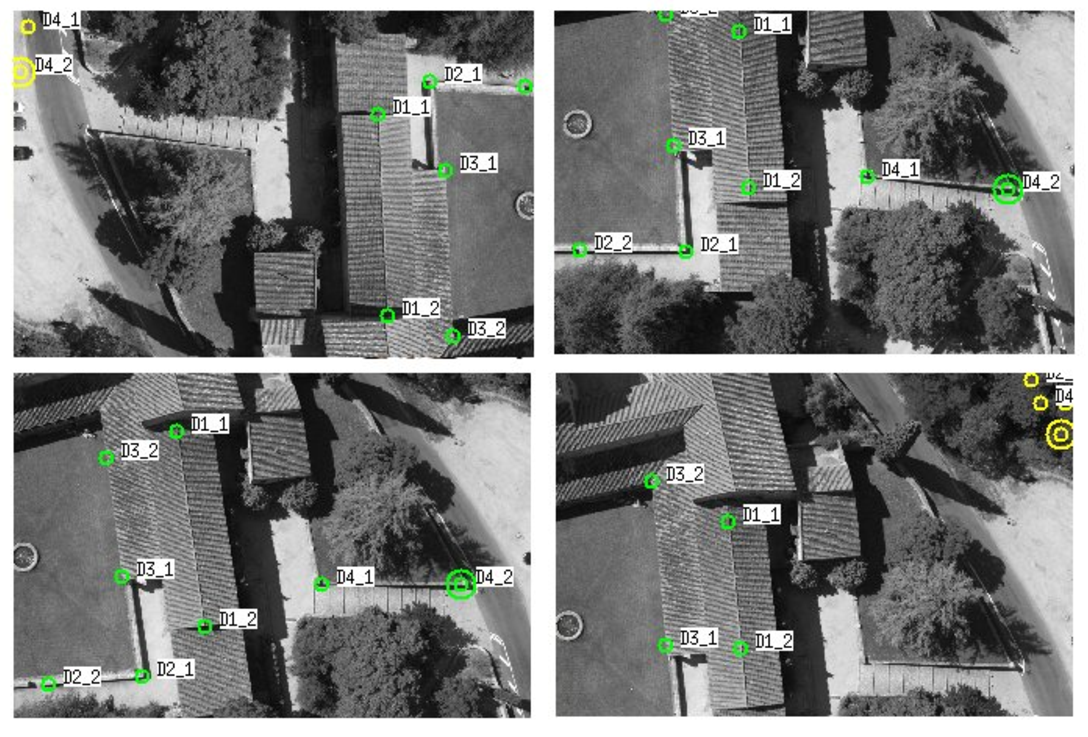
\includegraphics[width=120mm]{FIGS/Cuxa/linesSaisieAppuisInit1.pdf}
	\end{center}
	\caption{2D points acquisition with SaisieAppuisInit tool.}
\end{figure}

\noindent Hereafter, we will only be interested in the output file \texttt{mesures-S2D.xml} which contains pixel coordinates of $P_{ij}^1$ and $P_{ij}^2$ end points. Note that \texttt{mesures-S3D.xml} is either empty (when NONE argument has been provided as input orientation) or otherwise, does not contain any valuable information (since 3D coordinates are pseudo-intersection of non-homolgous points). Hence it can be discarded. We use \texttt{GCP2MeasuresL2D} tool to convert this 2D coordinate file to a 2D line file: \newline

\begin{verbatim}
mm3d GCP2MeasuresL2D mesures-S2D.xml 

Abbey-IMG_0173.jpg 3 line(s)
Abbey-IMG_0191.jpg 4 line(s)
Abbey-IMG_0192.jpg 4 line(s)
Abbey-IMG_0193.jpg 2 line(s)
-------------------------------------------------------------------------------
mesures-S2D.xml: 13 line(s) found in 4 image(s) -> L2D_mesures-S2D.xml
-------------------------------------------------------------------------------
\end{verbatim}

\noindent As a result, if no output name is specified, file \texttt{L3D\_<input\_name>.xml} is created.\newline

{\scriptsize
\begin{verbatim}
<?xml version="1.0" ?>
    <Xml_SetMeasureGlob3DLine>
        <AllMeasures>
            <NameIm>Abbey-IMG_0173.jpg</NameIm>
            <Measures>
                <NameLine3D>D1</NameLine3D>
                <P1>987.73286945994812 274.982879240555803</P1>
                <P2>1011.28698974809959 821.946130239705212</P2>
            </Measures>
            <Measures>
            <Measures>
                <NameLine3D>D2</NameLine3D>
                <P1>1126.34717028688192 186.860623522069659</P1>
                <P2>1382.99509794605456 201.237007364946635</P2>
            </Measures>
            <Measures>
                <NameLine3D>D3</NameLine3D>
                <P1>1167.2650377369323 426.889570999637954</P1>
                <P2>1189.27960700523249 876.110377648758913</P2>
            </Measures>
        </AllMeasures>
        <AllMeasures>
            <NameIm>Abbey-IMG_0191.jpg</NameIm>
            <Measures>
            ...
\end{verbatim}
}

\noindent To read this new file \texttt{L2D\_mesure-S2D.xml} programmatically, we call \texttt{StdGetFromSI} in C++ code: \newline


\begin{verbatim}
cXml_SetMeasureGlob3DLine M = StdGetFromSI("L2D_mesure-S2D.xml",SetMeasureGlob3DLine);
\end{verbatim}

\begin{figure}
	\begin{center}
		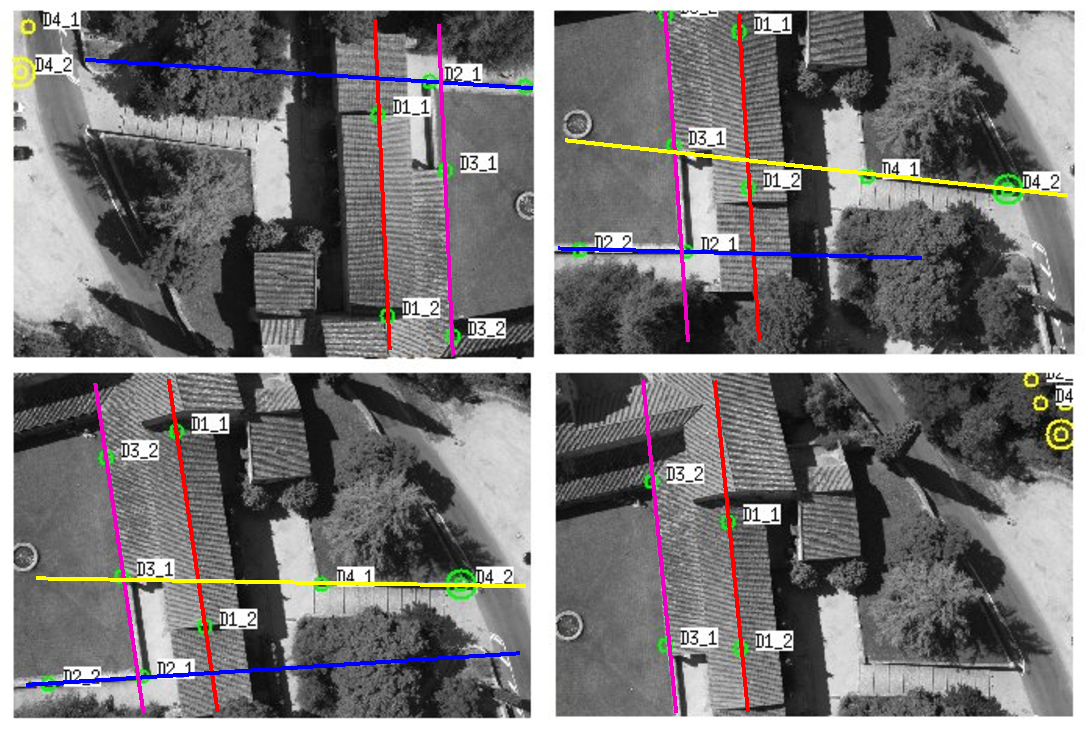
\includegraphics[width=120mm]{FIGS/Cuxa/linesSaisieAppuisInit2.pdf}
	\end{center}
	\caption{Result of \texttt{GCP2MeasuresL2D}: 4 lines in 4 images, \texttt{D1}, \texttt{D2}, \texttt{D3} and \texttt{D4} }
\end{figure}

\vspace{1cm}


\subsubsection{Conversion to 3D lines in space}

\noindent The tool \texttt{MeasuresL2D2L3D} can be used to compute an initial 3D line in orientation space. \newline

\begin{verbatim}
*****************************
*  Help for Elise Arg main  *
*****************************
Mandatory unnamed args : 
* string :: {2D Line measurement xml file}
* string :: {Orientation directory}
Named args : 
* [Name=3D Line output xml file] string
\end{verbatim}
\vspace{0.3cm}

\noindent Output file is an xml file containing a \texttt{cXml\_Set3DLine} type of object. An object \texttt{cXml\_Set3DLine} contains a member value \texttt{AllLines}, a list of \texttt{cXml\_One3DLine}, each of them containing the information relative to a 3D line in space : its name \texttt{NameLine3D}, an arbitrary reference point \texttt{Pt} (when there is no ambiguity, this point is defined as the intersection between the line and the $z=0$ plane) and a unit direction vector \texttt{Vec}. The output line parameters are refered to the input orientation. \newline

\begin{verbatim}
mm3d MeasuresL2D2L3D L2D_mesures-S2D.xml Ori-All-Rel/
\end{verbatim}
\vspace{0.3cm}

\noindent Currently, the 3D lines are computed with an empirical version of RANSAC algorithm, developped with Paul Chapron. Intersections of the "bundle planes" issued from two images where the line is visible are computed, hence for each pair of images, a line candidate is generated. This line is then compared with individual bundles issued from all other images where it is visible. A total root mean square error score $\rho$ is computed based on the geometric 3D residuals of pseudo-intersections between candidate lines and bundles. All line candidates with residual above $Z \times \rho$ (where $Z$ is a parameter, set to $1.0$ by default) are removed from the observation dataset. The remaining lines are then digitized with 100 points $\mathbf{x}_i \in \mathbb{R}^3$: \newline

$$\mathbf{x}_i = (1-\lambda_i) \mathbf{P}_1   + \lambda_i \mathbf{P}_2 
~~~~~~~~ \mbox{with:} ~~~~~~~~  \lambda_i = \frac{i}{100}$$ \newline

\noindent where $\mathbf{P}_1$ and $\mathbf{P}_2$ denote extremal intersections between bundles and line candidate. The digitization process provides $100 \times L$ 3D points for each line, where $L$ is the number of line candidates. When no candidate has been removed during the outlier search process, this number is equal to: \newline

$$L = \frac{M(M+1)}{2}$$ \newline

\noindent where $M$ is the number of images viewing the 3D line. \newline

\noindent The line direction is then estimated with a principal component analysis (PCA) on the digitized points. Since we are only interested in finding the eigen vector associated to the largest eigen value of the covariance matrix $\mathbf{\Sigma}$, we use the \textit{power iteration} method with convergence speed proportional to the ratio between the largest two eigen values (which makes this method particularly suitable in our case). The process is initiated with an arbitrary unit vector $\mathbf{x}^{(0)} = (1,0,0)^{T}$. The following iterations are performed until convergence (with $\mathbf{\Sigma} \in \mathbb{R}^{3 \times 3}$, convergence is usually reached with a couple of iterations) : \newline

$$\mathbf{x}^{(n+1)} = \frac{\mathbf{\Sigma}\mathbf{x}^{(n)}}{||\mathbf{\Sigma}\mathbf{x}^{(n)}||_2}$$ \newline

\noindent After convergence, $\mathbf{x}^{(n)}$ contains the unit vector of the estimated 3D line. As a byproduct, the adjustment residual is readily available, by substracting the eigen value $||\mathbf{\Sigma}\mathbf{x}^{(n)}||$ from the total variance of the dataset, which is equal to the trace of the covariance matrix : \newline



$$\mbox{RMSE} = \Big(\mbox{Tr}(\mathbf{\Sigma})  -  ||\mathbf{\Sigma}\mathbf{x}^{(n)}||\Big)^{\frac{1}{2}}$$ \newline

\noindent Eventually, the reference point is estimated through the mean vector of digitized points. \newline 

\noindent In the near future, a more sophisticated algorithm should be used to deal with more than only two observations at a time. In this second version, we may perform a global non-linear least squares adjustment between the unknown line and bundles. This solution will provide standard deviation paramaters for the 3D line estimations, which may pay off later as those lines are meant to be used as input prior solution to Campari algorithm.  \newline 


\begin{figure}[!h]
	\begin{center}
		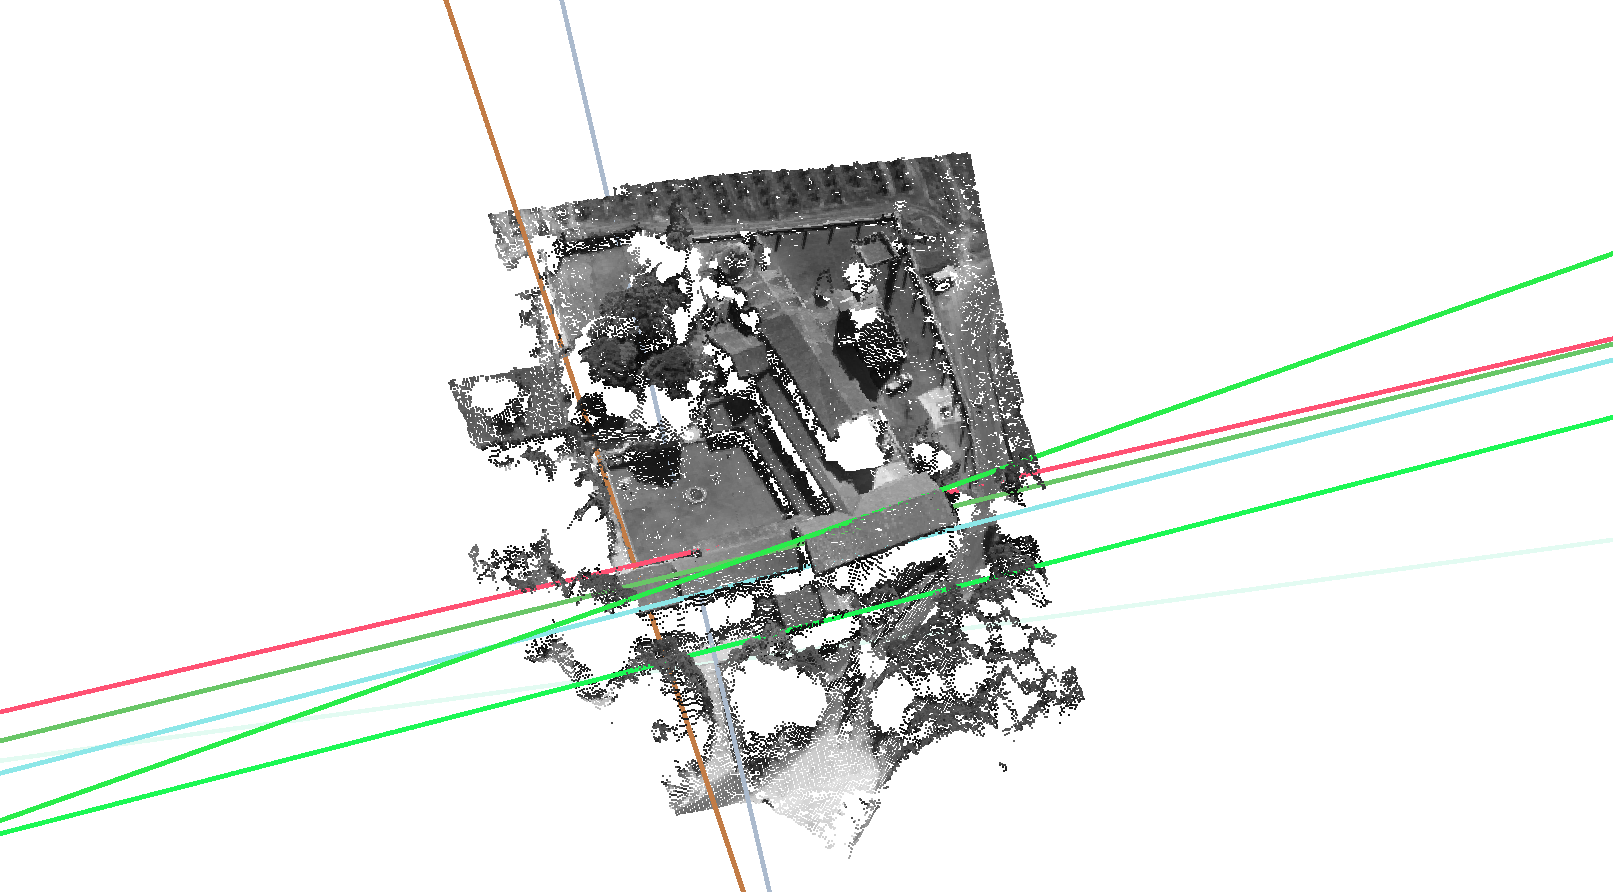
\includegraphics[width=140mm]{FIGS/Cuxa/linesWithMeshlab.png}
	\end{center}
	\caption{Result of \texttt{MeasuresL2D2L3D} and \texttt{L3D2Ply} for 8 lines on 4 images. }
\end{figure}


\noindent As a console output, the program displays the RMSE error for each pair of images and, for each 3D line, the select pair with lowest RMSE. The total RMSE is estimated a the square root of the sum of squares of individual RMSEs. It is provided in 3D ground units, at the end of the process. \newline



\begin{verbatim}
-----------------------------------------------------------------
IMAGE Abbey-IMG_0173.jpg 8 LINE MEASUREMENTS
IMAGE Abbey-IMG_0191.jpg 6 LINE MEASUREMENTS
IMAGE Abbey-IMG_0192.jpg 7 LINE MEASUREMENTS
IMAGE Abbey-IMG_0193.jpg 7 LINE MEASUREMENTS
-----------------------------------------------------------------
8 bundle observations for 3D line D1
Abbey-IMG_0173.jpg Abbey-IMG_0191.jpg  RMSE = 0.0023116
Abbey-IMG_0173.jpg Abbey-IMG_0192.jpg  RMSE = 0.00230208
Abbey-IMG_0173.jpg Abbey-IMG_0193.jpg  RMSE = 0.00254476
Abbey-IMG_0191.jpg Abbey-IMG_0192.jpg  RMSE = 0.0335992
Abbey-IMG_0191.jpg Abbey-IMG_0193.jpg  RMSE = 0.01574
Abbey-IMG_0192.jpg Abbey-IMG_0193.jpg  RMSE = 0.0273474
MIN: Abbey-IMG_0173.jpg Abbey-IMG_0192.jpg  RMSE = 0.00230208
-----------------------------------------------------------------
8 bundle observations for 3D line D2
Abbey-IMG_0173.jpg Abbey-IMG_0191.jpg  RMSE = 0.00276077
...
==================================================================
Output: 8 line(s) written in L3D_L2D_mesures-S2D.xml
Total RMSE = 0.00290502
==================================================================
\end{verbatim}
\vspace{0.3cm}

\noindent For example, with the 8 lines collected on \textit{Saint-Michel de Cuxa} dataset, the total root mean square error between candidate lines and bundles is 0.0029 ground units, which amounts to about 2.5 cm. \newline 


\noindent The output file (\texttt{L3D\_ + input\_file\_name} if not specified) can be transformed to a ply file with:

\begin{verbatim}
mm3d L3D2Ply L3D_L2D_mesures-S2D.xml
\end{verbatim}
\vspace{1cm}


\noindent Work in progress...

